\documentclass[../main.tex]{subfiles}

\graphicspath{{../images/}}

\begin{document}
\pagestyle{fancy}
\lhead{Lecture 5: 9/10/24}
\chead{Chapter 3.1-3.5}
\rhead{PHYS 463}

\section{Statistical thermodynamics}
\barh \vspace*{1em}

\subsection*{Irreversibility and attainment of equilibrium}

\subsection{Equilibrium conditions and constraints}

Equilibrium condition: The system is equally likely to be found in any accessible states.

``accessible states'': some specfic conditions/constraints of sysem , these limit the numebr of states the system can be possibly found.

Furthermore, how does the change of constraints change the number of accessible states?

\paragraph*{Examples:}

\begin{itemize}
    \item Box divided (partition) into two equal parts: left half is filled with gas, and the right half is empty. 
    After removing the partition (constraint), the gas spreads, but the probability of the gas being in the left half is much smaller, $\frac{1}{2^N}$. 
    Rather, we would expect an equal number of particles on each side for $N \to N_A$.
    \item Box with insulating wall constrained to move:
    If the barrier freely moves, we would expect the Pressures to equalize $P = P'$
    \item Box with noninsulating wall (can't move): We would expect temperature to be equal $T = T'$
\end{itemize}

After the states reach equilibrium, if we added the contraint back in, the system would not go back to the original state! (irreverssible process)

\paragraph*{But what is temperature???}
\begin{itemize}
    \item Kinetic energy? Heat transfer?
    \item Perhaps macroscopically: flow of heat from one system to another by touch (thermal contact)
\end{itemize}

\subsection{Distribution of energy between systems via heat} Consider two systems $A$ and $A'$:
\begin{itemize}
    \item $A$: Energy $E$, Number of states $\Omega(E)$
    \item $A'$: Energy $E'$, Number of states $\Omega(E')$
\end{itemize}
where $\Omega(E)$ is the \# of states in $A$ with energy range $(E, E+\delta E)$

The total combined system $A^{(0)}$, with number of states $\Omega^{(0)}$, has a constant total energy,
\[E^{(0)} = E + E' = \textrm{constant}\]
where we define: $\Omega^{(0)}(E)$: \# of states accessible to $A^{(0)}$ when the subsystem $A$ has energy $(E, E+\delta E)$.

When $A^{(0)}$ is in equilibrium the probability is proportional to the number of accessible states:
\[P(E) \propto \Omega^{(0)} (E), \qor P(E) = \frac{\Omega^{(0)}(E)}{\sum_E \Omega^{(0)} (E)} = C \Omega^{(0)}(E)\]
where $C$ is a constant.

\paragraph*{Multiplicity}
\begin{align*}
    \Omega^{(0)}(E) = \Omega(E) \Omega'(E^{(0)} - E)
\end{align*}
Now, the probability $P(E)$ with $E$ is 
\begin{align*}
    P(E) = C \Omega(E) \Omega'(E^{(0)} - E)
\end{align*}
Graphically, we would expect $E$ vs. $\Omega(E)$ to increase (as $E$ increases, $\Omega(E)$ increases), and same with $E'$ vs. $\Omega'(E')$. But $E$ vs. $\Omega'(E^{(0)} - E)$ would decrease.
In addition, the probability $P(E)$ as a function of $E$ would have a sharp peak near the equilibrium $\tilde E$.

\paragraph*{Finding maximum} Take the derivative (of the log because multiplication becomes addition):
\begin{align*}
    \pdv{\ln P(E)}{E} = 0, \quad \ln P(E) = \ln C + \ln \Omega(E) + \ln \Omega'(E^{(0)} - E)
\end{align*}
hence
\begin{align*}
    \pdv{\ln P(E)}{E} = \pdv{\ln(\Omega(E))}{E} - \pdv{\ln(\Omega'(E'))}{E'} = 0
\end{align*}

\paragraph*{Thermodynamic beta \href{https://en.wikipedia.org/wiki/Thermodynamic_beta}{(Wikipedia)}}
Define $\beta$:
\begin{align*}
    \beta = \pdv{\ln \Omega(E)}{E}
\end{align*}
where at equilibrium, \(\beta(\tilde E) = \beta'(\tilde E')\)

Then we introduce a \textit{dimensionless} parameter $T$ such that
\begin{align*}
    \boxed{k T = \frac{1}{\beta}}
\end{align*}
where $k$ ($k_B$ everywhere else) is the Boltzmann constant. Therefore, temperature characterizes the variation of density of state with energy.

\paragraph*{Entropy} From temperature and defining entropy $S(E)$:
\begin{align*}
    \frac{1}{T} = k\beta &= \pdv{k \ln \Omega(E)}{E}, \quad S(E) = k \ln\Omega (E) \\
    &= \pdv{S}{E}
\end{align*}

\paragraph*{Worksheet}
\begin{enumerate}
    \item \# of energy levels $\Phi_1(\epsilon) \leq \frac{\epsilon}{\Delta \epsilon} = C \epsilon$
    \item Average energy per molecule is $\epsilon = E/f$ (f molecules)
    \begin{align*}
        \Phi(E) = (\Phi_1(\epsilon))^f
    \end{align*}
    \item \begin{align*}
        \Omega(E) &= \Phi(E + \delta E) - \Phi(E) \\
        &= \pdv{\Phi(E)}{E} \delta E, = \Phi_1^{f-1} \pdv{\Phi_1}{\epsilon} \delta E
    \end{align*}
    \item If $f$ is very large
    \begin{align*}
        \ln \Omega &= (f-1) \ln\Omega(\epsilon) + \dots \\
        &\approx f\ln\Omega(\epsilon)
    \end{align*}
    \item So
    \begin{align*}
        \Omega \propto \phi_1(\epsilon)^f \propto E^f
    \end{align*}
\end{enumerate}

\newpage
\lhead{Lecture 6: 9/12/24}
\chead{Chapter 3.4-3.8}

\paragraph*{Review of last time:} What is temperature?

For two systems $A$ and $A'$ that present heat exchange:
\begin{itemize}
    \item $E^{(0)} = E + E'$: total energy is constant
    \item At thermal equilibrium, the temperature of the systems are the same.
    \item $P(E) \propto \Omega^{(0)}(E)$: probability of finding system $A$ to have energy $E$ is proportional to the number of accessible states in the total system $A^{0}$.
    \item $\Omega^{(0)}(E) = \Omega(E) \Omega'(E^{(0)} - E)$: multiplicity
    \item To find the maximum, take the derivative to zero:
    \begin{align*}
        \pdv{\ln P(E)}{E} &= 0 \\
        \implies \pdv{\ln \Omega(E)}{E} &= \pdv{\ln \Omega'(E^{(0)} - E)}{E'}
    \end{align*}
    where
    \begin{align*}
        \beta = \pdv{\ln \Omega(E)}{E} \quad \textrm{and} \quad kT = \frac{1}{\beta}
    \end{align*}
    and at equilibrium, $\beta(\tilde E) = \beta'(\tilde E')$
    Finally, we define entropy $S(E)$ as
    \begin{align*}
        S(E) = k \ln \Omega(E)
    \end{align*}
    where $S + S' =$ maximum at equilibrium
\end{itemize}
[insert figure graph of $P(E), \Omega(E), \Omega'(E')$]
\begin{figure*}[ht]
    \centering
    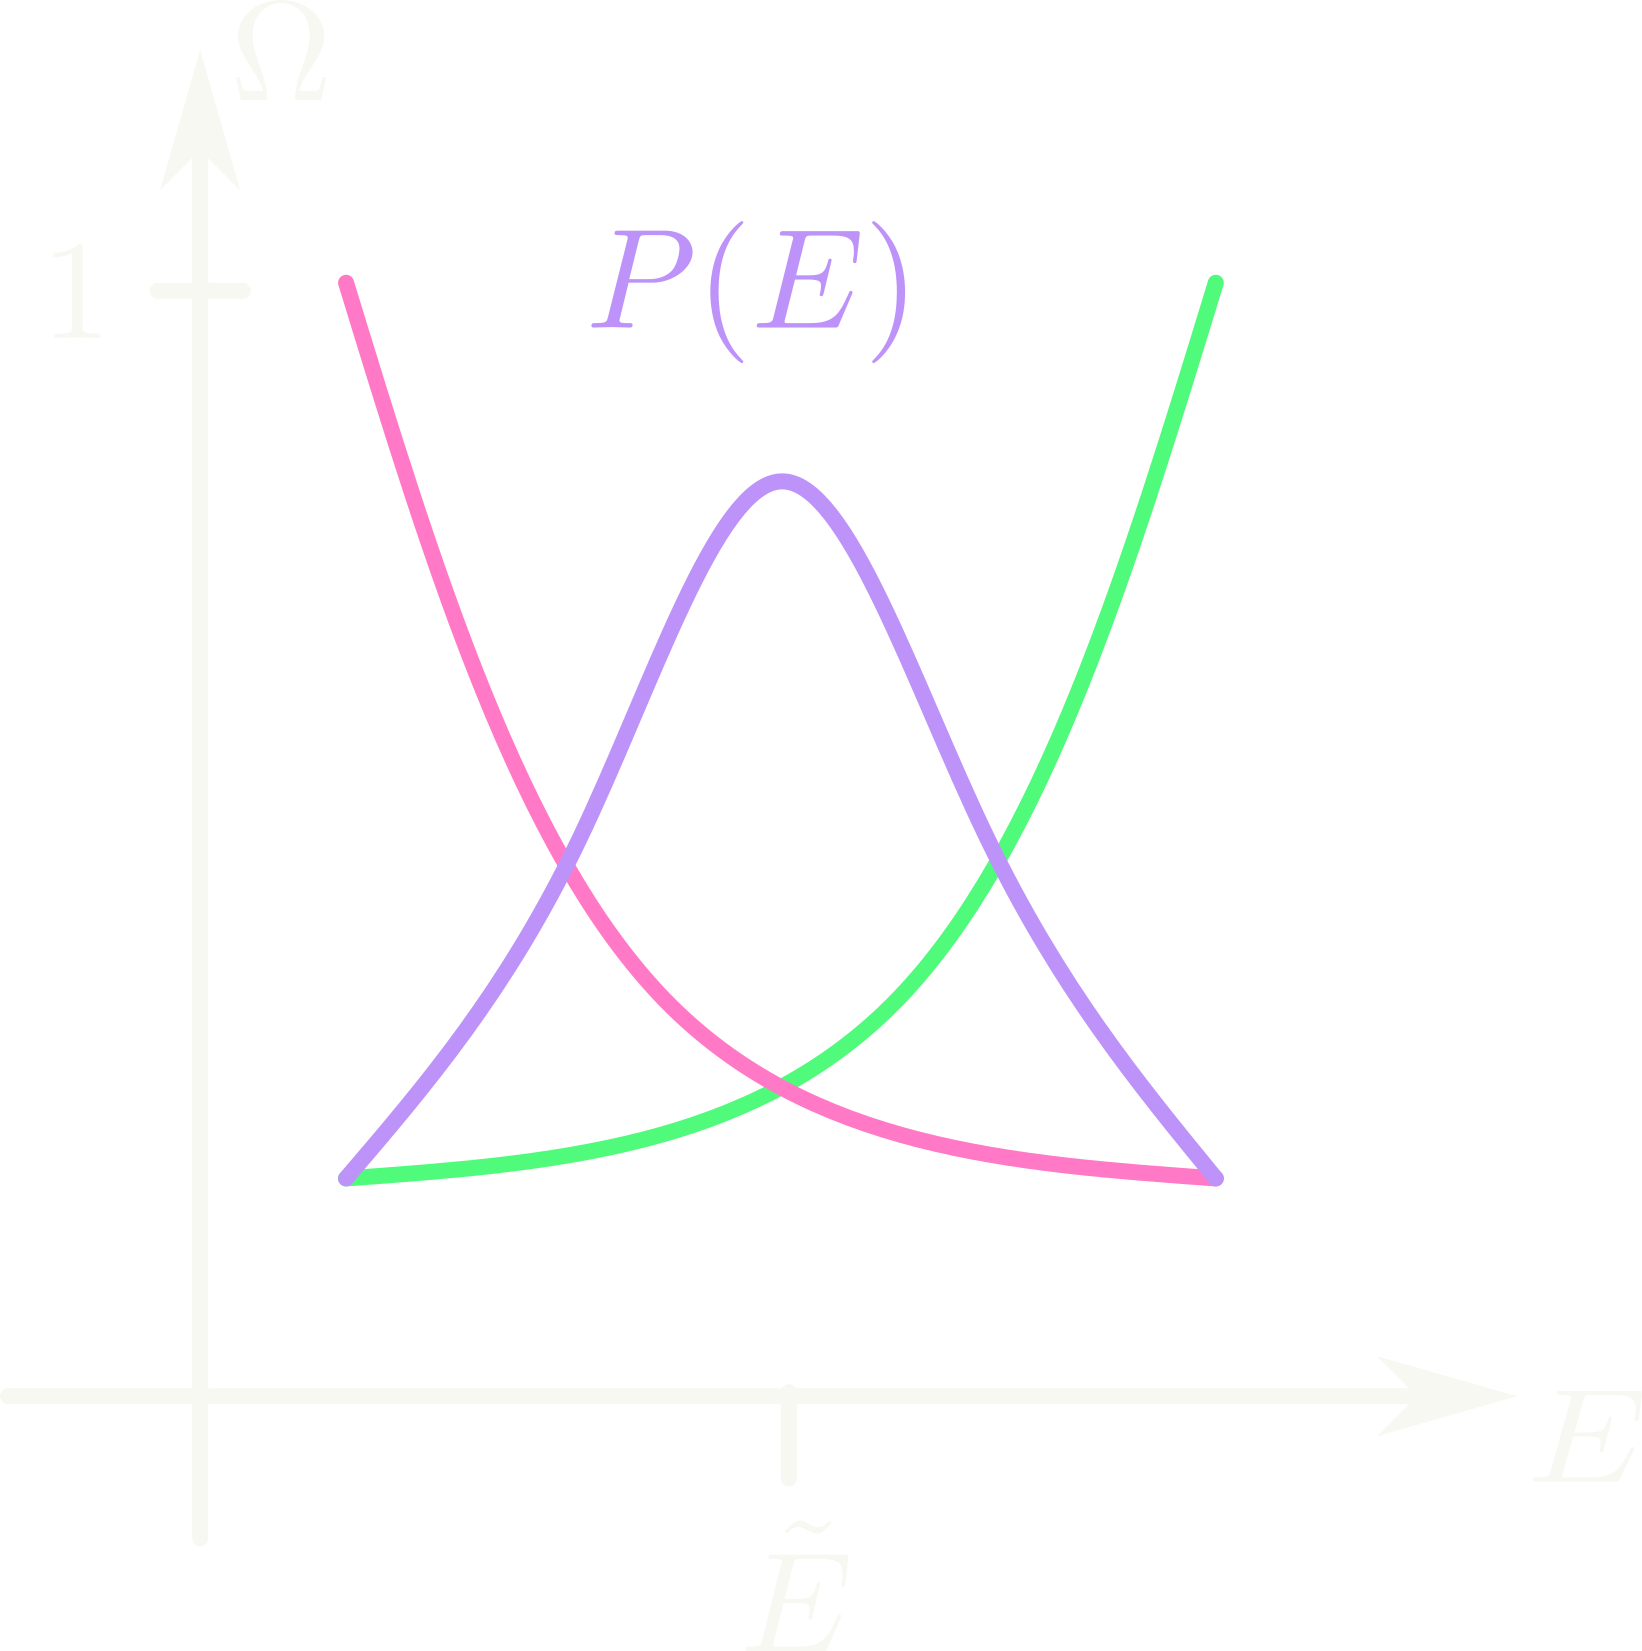
\includegraphics[width=0.3\linewidth]{fig3_1.png}
    \caption{Graph of $P(E), \Omega(E) \textrm{ (green)}, \Omega'(E')$}
    \label{fig:lecture3_1}
\end{figure*}
\paragraph*{What is} $kT$?

We replace $\Omega \sim E^f$ so
\begin{align*}
    \frac{1}{kT} &= \beta = \pdv{\ln \Omega}{E} \approx f \pdv{\ln E}{E} = \frac{f}{\bar E} \\
    \implies kT &\approx \frac{\bar E}{f}
\end{align*}
so $kT$ roughly represents energy per atom. Or

$kT$ is a measure of the mean energy above the ground state per atom

\begin{itemize}
    \item In the hydrogen atom, if $kT \geq \Delta$ (energy difference between the ground state and the first excited state), then the atom can be excited.
    \item Room temperature (300 K) is roughly $kT \approx 1/40$ eV $= 25$ meV
    \item A superconducting qubit of energy (usually in GHz) $\qty{25}{\micro eV}$ uses temperature in the magnitude of 15 mK:
    Backwards calculation: Going from 300K to 25 meV means we need to go to 0.3 K, but 0.03 K for the precision, to be in the range of the qubit.
\end{itemize}

\newpage
\subsection{Approach to equilibrium}

Given $A$, $A'$ we have average initial energy $\bar E_i$, $\bar E_i'$: At equilibrium
\begin{align*}
    \bar E_f &= \tilde E \\
    \bar E_f' &= \tilde E' = E^{(0)} - \tilde E
\end{align*}
The heat exchange is
\begin{align*}
    Q &= \bar E_f - \bar E_i \\
    Q' &= \bar E_f' - \bar E_i'
\end{align*}
where the total heat is constant, $Q + Q' = 0$.

\begin{itemize}
    \item The system that absorbs heat is ``colder''
    \item The system that releases (gives off) heat is ``hotter''
\end{itemize}

\subsection{Temperature}

Properties of $T$:
\begin{itemize}
    \item If the two systems have same $T$, they will remain in equilibrium when brought together.
    \item Zeroth Law of Thermodynamics: 
    If two systems are in thermal equilibrium with a 3rd system, then they must be in equilibrium with each other.

    This allows us to use a test system as a ``thermometer'':
    a small system that has a macroscopic parameter that varies when brought into contact with another system.
\end{itemize}

\subsection{Heat Reservoir}

A heat reservoir $A'$ with temp $T'$ transfers heat to a smaller system $A$ with temp $T$:
\begin{itemize}
    \item $T \to T'$
    \item $T'$ does not change!
\end{itemize}
Using the parameter $\beta' = \beta'(E')$ (where it is inversely related to temp), 
\begin{align*}
    \abs{\pdv{\beta'}{E'} Q'} \ll \beta'
\end{align*}
which pretty much tells us that $\Delta \beta' \ll \beta'$, so the temperature of the reservoir does not change.

The change of the density of states of the reservoir is
\begin{align*}
    \ln\Omega'(E' + Q') - \ln\Omega'(E') 
\end{align*}
where the Taylor expansion gives us
\begin{align*}
    = \pdv{\ln\Omega'}{E'} Q' = \beta' Q'
\end{align*}
This is proportional to the change of entropy:
\begin{align*}
    \Delta S' &= k(\ln\Omega'(E' + Q) - \ln\Omega'(E')) \\
    \beta'Q'k &= \frac{Q'}{T'}
\end{align*}
Simply,
\begin{align*}
    \Delta S' = \frac{Q'}{T'} \qqtext{(for a heat reservoir)}
\end{align*}
If one assumes an infinitesimal amount of heat $\dbar Q$
\begin{align*}
    \boxed{d S' = \frac{\dbar Q'}{T'}}
\end{align*}
which is the 2nd law of thermodynamics.

The first law of thermodynamics is (as we discovered)
\begin{align*}
    d E + \dbar W = \dbar Q
\end{align*}

\subsection{Dependence on Density of States (DoS) on external parameters}

$\Omega(E, x)$ where $x$ is an external parameter. The change of energy is
\begin{align*}
    \pdv{E}{x} dx \qqtext{where} X = -\pdv{E}{x} \qqtext{``generalized force''}
\end{align*}

\end{document}